\section{Finite Elements}

\numericsubsection{Variational Problem: Method of Ritz}

Having a two-point boundary problem $-u''(x) = f(x)$ with $v(0)=v(1)=0$ on $[0,1]$, we need to find a function
that minimises the functional $\phi(v) = \int_0^1\sfrac{1}{2}\cdot v'(x)^2-f(x)\cdot v(x)\ dx$

Idea of Ritz: Focusing on a vector subspace $\mathbb{V}^{(n)}\subset \mathbb{V}$ in which we know
that there's a solution and then minimise the functional for all linear combinations:
\begin{align*}
    a_1v_1(x)+\ldots+a_nv_n(x),\quad a_k\in\mathbb{R}
\end{align*}

We have the Ritz matrix
\begin{align*}
    R_{j,k}^{(n)} & = \int_0^1 v_j'(x)\cdot v_k'(x)\ dx \\
    & = v_j'(x)\cdot v_k(x)|_0^1 - \int_0^1 v_j''(x)\cdot v_k(x)\ dx \\
    & = - \int_0^1 v_j''(x)\cdot v_k(x)\ dx\quad\text{\color{gray} (homogeneous b.c.)}
\end{align*}
and the Ritz Vector
\begin{align*}
    r_k^{(n)} = \int_0^1 f(x)\cdot v_k(x)\ dx
\end{align*}
to find the $a$ coefficients: $R^{(n)}\cdot\vec{a} = \vec{r}^{(n)}$.

\subsubsection{Example}

\textbf{Given} Baby Poisson $-u''(x) = f(x)$ with ${\color{blue}f(x) = \pi^2\sin(\pi x)}$ with $u(0) = u(1) = 0$.
We want to compute the coefficient $b$ in the ansatz $\utild(x) = b\cdot(x - 2x^2 + x^3)$.

\textbf{Solution} We compute the (1-dimensional) Ritz matrix $R$ with
${\color{red} v1(x) = x - 2x^2 + x^3}$:
\begin{align*}
    R_{11} = \int_0^1 {\color{red}v_1}'(x)\cdot {\color{red}v_1}'(x)\ dx = \int_0^1 {\color{red}(1-4x+3x^2)}^2\ dx = \sfrac{2}{15}
\end{align*}

and the (1-dimensional) Ritz vector with
\begin{align*}
    r_1=\int_0^1 {\color{blue} f(x)}\cdot {\color{red}v_1(x)}\ dx = \int_0^1 {\color{blue} \pi^2\sin(\pi x)}\cdot{\color{red}(x-2x^2+x^3)}\ dx = \frac{2}{\pi}
\end{align*}

Thus, we get $R_{11}\cdot b = r_1$ and therefore $b=\sfrac{15}{\pi}$.

\numericsubsection{Method of Galerkin}

Weak reformulation: Find a function $u(x)$ (for problem $-u''(x)=f(x)\Rightarrow u''(x)+f(x)=0$) in $\mathbb{V}$ such that for all $v(x)\in\mathbb{V}$ one has
\begin{align*}
    \int_0^1 \left(u''(x) + f(x)\right)\cdot v(x)\ dx = 0
\end{align*}
and then focus on $n$ carefully chosen functions $v_1(x),\ldots,v_n(x)$ and find a function $\utild(x)$ in $\mathbb{V}^{(n)}$,
called ansatz, (that already satisfy the Dirichlet boundary conditions) such that, when substituted for the above integral
\begin{align*}
    \int_0^1 \left(\utild''(x) + f(x)\right)v_k(x)\ dx = 0,\quad {\color{gray} k = 1,\ldots,n}
\end{align*}

The $n$ equations thus turn into $n$ linear equations
\colorbox{shadecolor}{$
    \displaystyle
    \int_0^1 \left(a_1\cdot v_1''(x)+\ldots+a_n\cdot v_n''(x) + f(x)\right)\cdot v_k(x)\ dx = 0
$}

\colorbox{shadecolor}{for $k = 1,\ldots,n$},
giving the Galerkin Matrix $G_{k,j}^{(n)} = \int_0^1 v_j''(x)\cdot v_k(x)\ dx$ and the
Galerkin vector $g_k^{(n)} = \int_0^1 f(x)\cdot v_k(x)\ dx$ and the system $G^{(n)}\cdot\vec{a} + \vec{g}^{(n)} = 0$.
We can also observe that $G^{(n)} = -R^{(n)}$ and $\vec{g}^{(n)} = \vec{r}^{(n)}$.

\subsubsection{Example}

\textbf{Given} The function $u(x)$ on $\Omega = [0,1]$ satisfies Helmholtz's equation
$u''(x) + 17u(x) = 0$ (\emph{= 0 important, move to left side}) with Dirichlet conditions
$u(0) = 0, u(1) = 1$. Determine an approx. function $\utild(x)$ for $u(x)$ with the ansatz
$\utild(x) = x + a_1(x-x^2) + a_2(x^2-x^3)$ (that already satisfies b.c.)

\textbf{Solution}
Given the ansatz
\begin{align*}
    \utild(x) & = x + a_1{\color{blue}(x-x^2)} + a_2{\color{blue}(x^2-x^3)} \\
    \utild''(x) &  = -2a_1 + a_2(2-6x) \\
    {\color{blue} v_1(x)} & {\color{blue} = x-x^2} \\
    {\color{blue}v_2(x)} & {\color{blue}= x^2 - x^3}
\end{align*}
we receive the linear system
\begin{align*}
    & \int_0^1 \left(\utild''(x) + 17\utild(x)\right)\cdot {\color{blue}v_1(x)}\ dx = 0 \\
    & \int_0^1 \left(\utild''(x) + 17\utild(x)\right)\cdot {\color{blue}v_2(x)}\ dx = 0
\end{align*}

which gives
\resizebox{\columnwidth}{!}{$
    \displaystyle
    \int_0^1 \left[-2a_1 + a_2(2-6x) + 17(x + a_1{\color{blue}(x-x^2)} + a_2{\color{blue}(x^2-x^3)})\right]\cdot
    {\color{blue}(x-x^2)}\ dx = 0
$}
\resizebox{\columnwidth}{!}{$
    \displaystyle
    \int_0^1 \left[-2a_1 + a_2(2-6x) + 17(x + a_1{\color{blue}(x-x^2)} + a_2{\color{blue}(x^2-x^3)})\right]\cdot
    {\color{blue}(x^2-x^3)}\ dx = 0
$}

separating by coefficients:
\resizebox{\columnwidth}{!}{$
    \displaystyle
    \int_0^1 \left[a_1(-2+17x-17x^2) + a2(2-6x+17x^2-17x^3)\right]\cdot
    {\color{blue}(x-x^2)}\ dx = 0
$}
\resizebox{\columnwidth}{!}{$
    \displaystyle
    \int_0^1 \left[-2a_1 + a_2(2-6x) + 17(x + a_1{\color{blue}(x-x^2)} + a_2{\color{blue}(x^2-x^3)})\right]\cdot
    {\color{blue}(x^2-x^3)}\ dx = 0
$}

leaves a system in the form $a_1\int_0^1\cdots + a_2\int_0^1\cdots + \int_0^1\cdots = 0$. With the integrals solved, we get:
\begin{align*}
    a_1 \frac{7}{30} + a_2\frac{7}{60} + \frac{17}{12} = 0 \\
    a_1 \frac{7}{60} + a_2\frac{1}{85} + \frac{17}{12} = 0
\end{align*}

and we receive $a_1 \approx -8.45$ and $a_2 \approx 4.76$ and thus
$\utild(x) = x - 8.45 (x-x^2) + 4.76(x^2 - x^3)$.

\numericsubsection{Elliptic}

\makebox[\columnwidth]{\includegraphics[width=0.5\columnwidth]{images/FEM_Geometry}}

Introduce on problem domain nodal points that divide the geometry into cells or meshes.
Associate to each nodal variable $a_k$ of a nodal point a local function $v_k$ from 
a set of given local basis functions $v_1(x), \ldots, v_n(x)$ that are continuous and piecewise differentiable.
Thus, the ansatz $\utild(x) = a_0v_0(x)+a_1v_1(x)+\ldots+a_nv_n(x)$ has shape functions $v_k$ that are one on
the respective nodal point $k$.
Then, we use shape functions to represent the PDE on the mesh,
e.g. using triangular functions $l_1(x)=1-x$ and $l_2(x) = x$ to obtain \emph{local} element matrices
\begin{snugshade*}
\begin{align*}
	E_\text{step} = 
	\begin{bmatrix}
		\int_0^1 l_1^\prime(s)\cdot l_1^\prime(s)\ ds & \int_0^1 l_1^\prime(s)\cdot l_2^\prime(s)\ ds \\
		\int_0^1 l_2^\prime(s)\cdot l_1^\prime(s)\ ds & \int_0^1 l_2^\prime(s)\cdot l_2^\prime(s)\ ds
	\end{bmatrix}
	=
	\begin{bmatrix}
		1 & -1 \\
		-1 & 1
	\end{bmatrix}
\end{align*}    
\end{snugshade*}


that can then be used to construct the mesh matrix $M=1/h\cdot E$ using mesh size $h$.
Afterwards, the global Ritz matrix can be computed, e.g. for a one-dimensional mesh with 4 nodal points and 2 unknown inner points,
yielding 4 base functions $v_1,v_2,v_3,v_4$:

\begin{align*}
	R^4 = \begin{bmatrix}
		{\color{red} M^{(1)}_{0,0}} & \color{red}{M^{(1)}_{0,1}} & 0 & 0 \\
		{\color{red} M^{(1)}_{1,0}} & {\color{red} M^{(1)}_{1,1}} + {\color{blue} M^{(2)}_{0,0}} & {\color{blue} M^{(2)}_{0,1}} & 0 \\
		0 & {\color{blue} M^{(2)}_{1,0}} & {\color{blue} M^{(2)}_{1,1}} + {\color{green} M^{(3)}_{0,0}} & {\color{green} M^{(3)}_{0,1}} \\
		0 & 0 & {\color{green} M^{(3)}_{1,0}} & {\color{green} M^{(3)}_{1,1}}
	\end{bmatrix}
\end{align*}

The system vector can then be calculated:

\begin{align*}
	\vec{r^4} = \begin{pmatrix}
		\int_0^1 f(x)\cdot v_0(x)\ dx \\
		\vdots \\
		\int_0^1 f(x)\cdot v_3(x)\ dx
	\end{pmatrix}
\end{align*}

Finally, we have obtained the Ritz system: $R^4\cdot\vec{a}=\vec{r^4}$.
That yields the approximation function (as defined by the ansatz): $\tilde{u}(x)=\sum_{i=0}^3 a_i\cdot v_i(x)$
with $a_0$ and $a_3$ fulfilling the boundary conditions.

This shape function approach can also be applied to the Ritz vector.
We get $\tilde{f}(x) = f(a_0)\cdot v_0(x)+\ldots+f(a_n)v_n(x)$ and we approximate 
$r_{k}^{n}=\int_{0}^{1}f(x)\cdot v_{k}(x)\;dx$ by $\tilde{r}_{k}^{n}=\int_{0}^{1}\tilde{f}(x)\cdot v_{k}(x)\;dx$
which essentially is $\tilde{r}^n = S^n \cdot \vec{f}^n$ where $\vec{f}^n$ is the vector of nodal values
and $S_{k,j}^n=\int_0^1 v_j(x)\cdot v_k(x)\ dx$

\subsubsection{Example With Inhomogeneous B.C.}

\textbf{Given} A real function $u(x)$ on interval $\Omega=[0,1]$ that satisfies the differential equation $u''(x) + 8 = 0$
and the boundary conditions $u(0) = 1$ and $u(1) = 2$. We want to find an approximation function $\utild(x)$ using the meshes
$[0, 0.5], [0.5, 0.75], [0.75, 1]$ and linear shape functions.
\\[1em]
\textbf{Discretisation of Geometry}
\makebox[\columnwidth]{\includegraphics[width=0.8\columnwidth]{images/FEM_Example}}

\textbf{Solution}

We get the following mesh matrices:

Mesh 1 (step size = 1/2):
\begin{align*}
    {\color{red}
    \frac{1}{h}\begin{bmatrix}
        1 & -1 \\
        -1 & 1
    \end{bmatrix}
    = \sfrac{1}{2}^{-1} \begin{bmatrix}
        1 & -1 \\
        -1 & 1
    \end{bmatrix}
    =
    \begin{bmatrix}
        2 & -2 \\
        -2 & 2
    \end{bmatrix}
    }
\end{align*}

Mesh 2 (step size = 1/4):
\begin{align*}
    {\color{blue}
    \frac{1}{h}\begin{bmatrix}
        1 & -1 \\
        -1 & 1
    \end{bmatrix}
    =
    \begin{bmatrix}
        4 & -4 \\
        -4 & 4
    \end{bmatrix}
    }
\end{align*}

Mesh 3 (step size = 1/4):
\begin{align*}
    {\color{green}
    4\begin{bmatrix}
        1 & -1 \\
        -1 & 1
    \end{bmatrix}
    =
    \begin{bmatrix}
        4 & -4 \\
        -4 & 4
    \end{bmatrix}
    }
\end{align*}

resulting in the global Ritz-Matrix and Ritz-Vector:

\begin{align*}
    & \overbrace{
        \begin{bmatrix}
            {\color{red}2} & {\color{red}-2} & 0 & 0 \\
            {\color{red}-2} & {\color{red}2} + {\color{blue}4} = 6 & {\color{blue}-4} & 0 \\
            0 & {\color{blue}-4} & {\color{blue}4} + {\color{green}4} = 8 & {\color{green}-4} \\
            0 & 0 & {\color{green}-4} & {\color{green}4}
        \end{bmatrix}
    }^R
    \overbrace{
        \begin{bmatrix}
            a_0 \\
            a_1 \\
            a_2 \\
            a_3
        \end{bmatrix}
    }^{\vec{a}}
    =
    \overbrace{
        \begin{bmatrix}
            \int_0^1 f(x)v_0(x)\ dx \\
            \int_0^1 f(x)v_1(x)\ dx \\
            \int_0^1 f(x)v_2(x)\ dx \\
            \int_0^1 f(x)v_3(x)\ dx
        \end{bmatrix}
    }^{\vec{r}} \\
    & = 
    \begin{bmatrix}
        \frac{\sfrac{1}{2}\cdot 8}{2} = 2\quad\text{(area of {\color{red} red shape function})} \\
        \frac{\sfrac{3}{4}\cdot 8}{2} = 3\quad\text{(area of {\color{blue} blue shape function})} \\
        \frac{\sfrac{1}{2}\cdot 8}{2} = 2\quad\text{(area of {\color{violet} violet shape function})} \\
        \frac{\sfrac{1}{4}\cdot 8}{2} = 1\quad\text{(area of {\color{green} green shape function})} \\
    \end{bmatrix}
\end{align*}

to satisfy inhomogeneous boundary conditions, we set $a_0$ and $a_3$ to the boundary condition in the vector $\vec{a}$ and
eliminate the corresponding equations, leading to the reduced Ritz system:

\begin{align*}
    \begin{bmatrix}
        -2 & 6 & -4 & 0 \\
        0 & -4 & 8 & -4
    \end{bmatrix}
    \begin{bmatrix}
        1\;\text{\color{gray} (b.c.)} \\
        a_1 \\
        a_2 \\
        2\;\text{\color{gray} (b.c.)}
    \end{bmatrix}
    = \begin{bmatrix}
        3 \\ 2
    \end{bmatrix}
\end{align*}
meaning
\begin{align*}
    \begin{bmatrix}
        6 & -4 \\
        -4 & 8
    \end{bmatrix}
    \begin{bmatrix}
        a_1 \\ a_2
    \end{bmatrix}
    +
    \begin{bmatrix}
        -2 \\ -8
    \end{bmatrix}
    =
    \begin{bmatrix}
        3 \\ 2
    \end{bmatrix}
\end{align*}

giving $a_1 = \sfrac{5}{2}$ and $a_2 = \sfrac{5}{2}$.

\subsubsection{Example With Homogeneous Boundary Conditions}

\textbf{Given} the differential equation $u''(x) + 1 = 0$ on $\Omega = [0,1]$ with homogeneous boundary conditions.
We want to approximate using meshes $[0,0.25], [0.25, 0.75], [0.75, 1]$.
\\[1em]
\textbf{Discretisation of Geometry}

Since we have homogeneous boundary conditions, we can ignore $v_0$ and $v_3$:
\makebox[\columnwidth]{\includegraphics[width=0.4\columnwidth]{images/FEM_Example2}}
giving $\utild(x) = 0 v_0(x)+a_1v_1(x)+a_2v_2(x)+0v_3(x)$.
\\[1em]
\textbf{Solution}

For steps 1, 2 and 3, we get the mesh matrices
\begin{align*}
    M_1 = 4\cdot E, M_2=2\cdot E, M_3 = 4\cdot E
\end{align*}
using element matrix $E$ of step function and thus the Ritz matrix
\begin{align*}
    R=\begin{bmatrix}
        4 & -4 & 0 & 0 \\
        -4 & 6 & -2 & 0 \\
        0 & -2 & 6 & -1 \\
        0 & 0 & -4 & 4
    \end{bmatrix}
\end{align*}

due to homogeneous boundary conditions, we cancel the first and last row and columns, resulting in the reduced Ritz system:
\begin{align*}
    \begin{bmatrix}
        6 & -2 \\
        -2 & 6
    \end{bmatrix}
    \begin{bmatrix}
        a_1 \\ a_2
    \end{bmatrix}
    =
    \begin{bmatrix}
        \sfrac{3}{8} \\ \sfrac{3}{8}
    \end{bmatrix}
\end{align*}

\subsubsection{Example With Funky $f(x)$}

Problem: $-u''(x) = f(x)$ in $\Omega = [0,1]$ with
\begin{align*}
    f(x) = \left\{
    \begin{array}{ll}
        8 & \text{if } x\in [0,\sfrac{1}{4}), \\
        24 & \text{if } x\in [\sfrac{1}{4},\sfrac{1}{2}), \\
        40 & \text{if } x\in [\sfrac{1}{2},\sfrac{3}{4}), \\
        16 & \text{if } x\in [\sfrac{3}{4},1),
    \end{array}
    \right.
\end{align*}
and homogeneous b.c. and $h = 1/4$.

\makebox[\columnwidth]{\includegraphics[width=0.5\columnwidth]{images/FEM_Example3}}

The Ritz vector then is:

For $v_1$: $8\cdot\frac{1}{4}\frac{1}{2} = 1$; $24\cdot \frac{1}{4}\frac{1}{2} = 3\rightarrow 1+3=4$

For $v_2$: $24\cdot\frac{1}{4}\frac{1}{2} = 3$; $40\cdot \frac{1}{4}\frac{1}{2} = 5\rightarrow 3+5=8$

For $v_3$: $40\cdot\frac{1}{4}\frac{1}{2} = 5$; $16\cdot \frac{1}{4}\frac{1}{2} = 2\rightarrow 5+2=7$

\numericsubsection{p-Strategy}

Using quadratic shape functions $q_1(x) = (1-x)(1-2x), q_2(x) = 4x(1-x), q_3(x) = -x(1-2x)$ as shape functions

\makebox[\columnwidth]{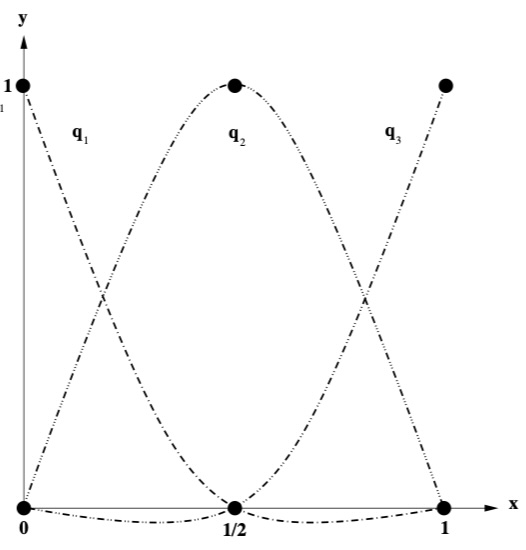
\includegraphics[width=0.4\columnwidth]{images/FEM_pStrategy}}

The v-functions for three nodes then look like

\makebox[\columnwidth]{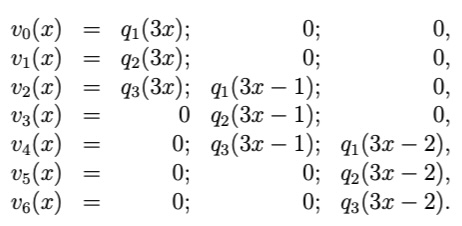
\includegraphics[width=0.5\columnwidth]{images/FEM_v_functions}}

with an affine transformation of the x values onto the nodal points.

We get a new element matrix:
\begin{snugshade*}
    \begin{align*}
        E = 
        \begin{bmatrix}
            7 & -8 & 1 \\
            -8 & 16 & -8 \\
            1 & -8 & 7
        \end{bmatrix}
    \end{align*}
\end{snugshade*}

and the associated mesh matrix $M = 1/h\cdot E$.
The Ritz vector can be computed analogous to the previous methods:
\begin{align*}
    \vec{r} = \begin{bmatrix}
        \int_0^1 f(x)\cdot v_0(x)\ dx \\
        \int_0^1 f(x)\cdot v_1(x)\ dx \\
        \vdots \\
        \int_0^1 f(x)\cdot v_n(x)\ dx
    \end{bmatrix}
\end{align*}

with the difference that the integral is not as straight forward as with the triangle function
({\color{blue}\faInfo}\ except for baby Laplace problem $u''(x) = 0$, since there the Ritz-vector is zero and no integration needed)
